% This is samplepaper.tex, a sample chapter demonstrating the
% LLNCS macro package for Springer Computer Science proceedings;
% Version 2.20 of 2017/10/04
%
\documentclass[runningheads]{llncs}
%
\usepackage{graphicx}
%\usepackage{ngerman}
\usepackage[utf8x]{inputenc}
\usepackage{fancyvrb}
\usepackage{courier}
\usepackage{helvet}
\usepackage{tikz}
\usepackage{xcolor}
\usepackage{pdfpages}
\usetikzlibrary{calc}
\usepackage[strict]{changepage}
\usepackage{xspace}
\usepackage{hyperref}
\usetikzlibrary{shapes.geometric}
\usetikzlibrary{arrows}
\usetikzlibrary{positioning}
\usetikzlibrary{arrows.meta, automata, shapes, matrix,positioning}
\usepackage{amssymb}
\usepackage{pifont}% http://ctan.org/pkg/pifont
\usepackage{subcaption} 
\usepackage{float}
\usepackage{fixfoot}
\usepackage{graphicx}
\usepackage{wrapfig}
\usepackage{multicol}
\usepackage{amsmath}
\usepackage{cleveref}
\usepackage{listings}
\setlength{\parindent}{0em}
\newcommand{\cmark}{\ding{51}}%
\newcommand{\xmark}{\ding{55}}%
% Used for displaying a sample figure. If possible, figure files should
% be included in EPS format.
%
% If you use the hyperref package, please uncomment the following line
% to display URLs in blue roman font according to Springer's eBook style:
% \renewcommand\UrlFont{\color{blue}\rmfamily}

\begin{document}
	
	
	%
	%	\title{Clustering Analysis of Mobility Data}
	\title{Are you moving predictably?}
	%
	%\titlerunning{Abbreviated paper title}
	% If the paper title is too long for the running head, you can set
	% an abbreviated paper title here
	%
	%TODO: Order by Lastname?
	\author{Miriam Wagner\and
		Martin Breuer\and
		Moritz Werthebach\and
		Timo Bergerbusch\and
		Walter Schikowski}
	%
	\authorrunning{T. Bergerbusch et al.}
	% First names are abbreviated in the running head.
	% If there are more than two authors, 'et al.' is used.
	%
	\institute{RWTH Aachen, Templergraben 55, 52062 Aachen, Germany}
	%
	\maketitle              % typeset the header of the contribution
	%
	\begin{abstract}
		We analyze movements in the urban environment of the Columbian city Medellín. Each movement is given as spatiotemporal pattern of with additional information about the reason, means of transportation and the corresponding person like the socio-economic status (strata), the age and gender. 
		% Marías sentence
		The objective of the paper is twofold: try to find groups of movement patterns and see, whether they correspond to socio-economic status, and then, since we have the economic status of each person in the data set, we will apply supervised learning to classify patterns into socio-economic status.
%		Since in most cases we do not have information about the actual socio-economic status of persons we firstly try different unsupervised approaches to find natural clusters. Due to bad results we introduce our preprocessing steps and switch to supervised learning.		
		Decision trees and neural networks did neither match our performance expectations, which leads to our conclusion that we need more data and information about the data in order to find a proper social stratification and to predict the given socio-economic status accurately.
		
		\keywords{Data Mining \and Clustering \and Rapidminer \and Cluster \and Neural Nets}
	\end{abstract}
	%
	%
	%	
	\section{Introduction} \label{sec: introduction}
	% could add more in depth 
	Within the time of Industry 4.0 and various data sources the question arises, if one can define who we are by the collected data? In particular is it possible to determine the wealth of a person, only given movements of a single day?
	For this we considered the dataset stated in \cite{rich_do_not_rise_early}. There we have a set of 124979 rows of movement data of various persons from the Columbian town Medellín, which is the second largest Colombian town with an estimated population of 2.5 million as of 2017 \cite{population_number} . All the data was collected at a single day, with possibly multiple entries referring to the same person.\\
	The data entries consist of data about the movement, like endpoints, length, and also some meta parameters like gender, age or the so-called strata of the person. The strata defines the socio-economic group, reflecting the affluence and therefore impose the ancillary costs. Those costs are defined by Colombians laws, which classifies households to regulate the access to public utility services, having as a result six socio-economic strata \cite{rich_do_not_rise_early}.\\
	Our goal is to ascertain, if there is a correlation between the movements and the strata, in order to be able to predict the strata based on the movements. This is done in two steps:\\
	First, by clustering using the k-means algorithm, considering different distance measures, with optionally including the principal component analysis (PCA).\\
	And second, a decision tree and neural net were trained and tested.
	
	\section{Methods}
	
	\subsection{Preprocessing}\label{sec: proprocessing}
	In order to classify the given data into smaller test sets or mask different aspects, we have to perform some analysis.\\
	We observe that even though we have 124979 individual lines defining a movement, there is one line defining a \texttt{NotANumber}-exception and therefore gets neglected for further usage.	\\
	We provide the \texttt{testDataGenerator} python script. Through flags and input arguments, the script is able to create all test sets used by our clustering and neural net approaches.\\
	We observe the following distribution over the whole dataset:\\
	
	\vspace*{-3em}
	\begin{figure}[H]
		\centering		
		\setlength\tabcolsep{.2cm}
		\begin{tabular}{c|ccccccc}
			strata &  1   &   2   &   3   &  4   &  5   &  6   & $\Sigma$ \\ \hline
			abs   & 6963 & 52265 & 49404 & 8772 & 5536 & 2038 &  124978  \\
			\%   & 5.57 & 41.82 & 39.53 & 7.02 & 4.43 & 1.63 &   100
		\end{tabular}
		\vspace*{-2.5em}
		\label{table: distribution normal}
	\end{figure}
	There is an upper bound on equal distribution through strata 6. It has at most 2038 individual elements.
	Furthermore we have to make sure that two different data points, which belong to the very same person, are assigned to the same cluster. To do so, we compute the value \texttt{ID}, which identifies each person and can be used to combine movements that are considered to be from the same person. I.e. two movements correspond with the very same person, if and only if they are consecutive in the original dataset and have the same strata, age and gender. This approach is taken since the surveys are concatenated sequentially and it is unlikely, that multiple consecutive movements with same strata, age, gender belong to two different persons.\\
	
	\vspace*{-3em}
	\begin{figure}[H]
		\centering
		\setlength\tabcolsep{.2cm}
		\begin{tabular}{c|ccccccc}
			strata &  1   &   2   &   3   &  4   &  5   &  6  & $\Sigma$ \\ \hline
			abs   & 3153 & 23367 & 21418 & 3497 & 2083 & 595 &  54113   \\
			\%   & 5.83 & 43.18 & 39.58 & 6.46 & 3.85 & 1.1 &   100
		\end{tabular}
		\vspace*{-2.5em}
	\end{figure}
	Following, we introduce vectors representing single persons. Since strata 6 is the smallest strata with 595 persons, it limits the size of an equally distributed dataset where each data point coincides with one person.\\
	
	\textbf{Stratified Person Data}\label{subsubsec: person vector data}\\
	As stated before, instead of simple IDs for every person we expand the parsing by using a data encapsulating in a class called \texttt{Person}. This class stores the ID, the parameters defining a person (c.f. \Cref{sec: proprocessing}), and all movements from that person.\\
	Then we are able to compute the following vector, with 850 entries, for further usage, that combines all movements of the person:
	\begin{align*}
	\underbrace{\#o_1, \dots, \#o_{413}, \#d_1, \dots, \#d_{413}}_{2\cdot 413} ,
	\underbrace{\mathit{AM}, \mathit{MD}, \mathit{PM}, \mathit{MN}}_{4}, 
	\underbrace{\#r_1, \dots, \#r_7}_{7}, \\
	\underbrace{\#\mathit{MoT}_1, \dots, \#\mathit{MoT}_7}_{7}, \underbrace{\mathit{S_{Dest}}, \mathit{S_{Dist}}, \mathit{G}, \mathit{A} ,\mathit{strata}, \mathit{strataGrouped}}_{6}
	\end{align*}
	with the following abbreviations ($1 \le i \le 413$, $1 \le j \le 7$):
	\begin{figure}[H]
		\centering
		\hspace*{-.3cm}
		\begin{subfigure}{0.50\textwidth}
		\begin{itemize}
			\setlength{\itemindent}{.4cm}
			\item[$o_i$:]  the $i$-th origin data point
			\item[$d_i$:]  the $i$-th destination data point
			\item[$\mathit{AM}$:] movements at time stamp AM
			\item[$\mathit{MD}$:] movements at time stamp MD
			\item[$\mathit{PM}$:] movements at time stamp PM
			\item[$\mathit{MN}$:] movements at time stamp MN
			\item[$r_j$:] the $j$-th reason
		\end{itemize}
	\end{subfigure}\hspace*{1cm}
	\begin{subfigure}{0.48\textwidth}
	\begin{itemize}
			\item[$\mathit{MoT}_j$:] the $j$-th mean of transportation
			\item[$\mathit{S_{Dest}}$:] sum of all durations
			\item[$\mathit{S_{Dist}}$:] sum of all distances
			\item[$\mathit{G}$:] the gender
			\item[$\mathit{A}$:] the age
			\item[$strata$:] the strata (used for comparison)
			\item[$strataGrouped$:] the aggregated stratas
		\end{itemize}
	\end{subfigure}
	\end{figure}


	
	\subsection{Unsupervised learning}
	\subsubsection{Clustering the data}
	
	is in the field of \textit{Data Mining}, \textit{Cluster Analysis} or \textit{Clustering} a process of grouping data objects from a dataset into multiple groups. The essential criterion, for the quality of the clustering, is \textit{similarity}, such that data objects are similar to other objects in the same cluster and dissimilar to objects from other clusters. 
	
	In the scope of this work, we decided to use the well-known partitioning methods k-means. In general, given $n$ data objects partitioning methods distribute the data objects into $k$ clusters with $k\le n$, using a distance measure to evaluate the respective similarity. 
%	Those methods form exclusive clusters by ensuring that each cluster contains at least one object.
	Note that the number $k$ of clusters has to be chosen manually a-priori and given to the partitioning process.
	
	\subsubsection{k-Means}
	
	is a \textit{centroid based technique}, which means that each cluster is represented by a data point, that also is the centre of the cluster. A distance measure is then used to assign every remaining data object from the data set to the best fitting cluster. This is done according to its similarity to the centre of this cluster and its dissimilarity to the centres of any other cluster.
	
	The data objects within a dataset are considered to reside in a euclidean space. Thus, the euclidean distance is used to calculate a score for the similarity of two data points. When using k-Means, the quality of a cluster $C_i$ can be evaluated by computing the sum of squared errors between all data points $p$ in the object space and the centroids $c_i \in C_i$ of every cluster. This method is known as \textit{within-cluster variation} \cite{data_mining} and defined as follows: 
	\begin{equation}
		E = \sum_{i=1}^{k} \sum_{p \in C_i} dist(p, c_i)^2,
	\end{equation}
	Given $k$, the first step of k-Means is to select $k$ random points as cluster centres. Those do not have to be actual data points.
%	objects in the data set as initial representatives for the cluster centres.
	After that, each remaining data object is assigned to the best fitting cluster based on a similarity score between the data point and every cluster centre. The overall goal of k-Means clustering is to iteratively optimize the within-cluster variation. In order to achieve this, each cluster centroid is redefined as the mean of all objects within that cluster. By considering the updated centroids, every data point is reassigned to the now best fitting cluster. This iterative process will continue until no better clustering can be found.\\
%	\subsubsection{Clustering with RapidMiner}	
	As a tool we considered RapidMiner, since it has many modules already efficiently implemented and is easy to adapt.
	\vspace*{-2em}
	\begin{figure}[!htbp]
		\centering
		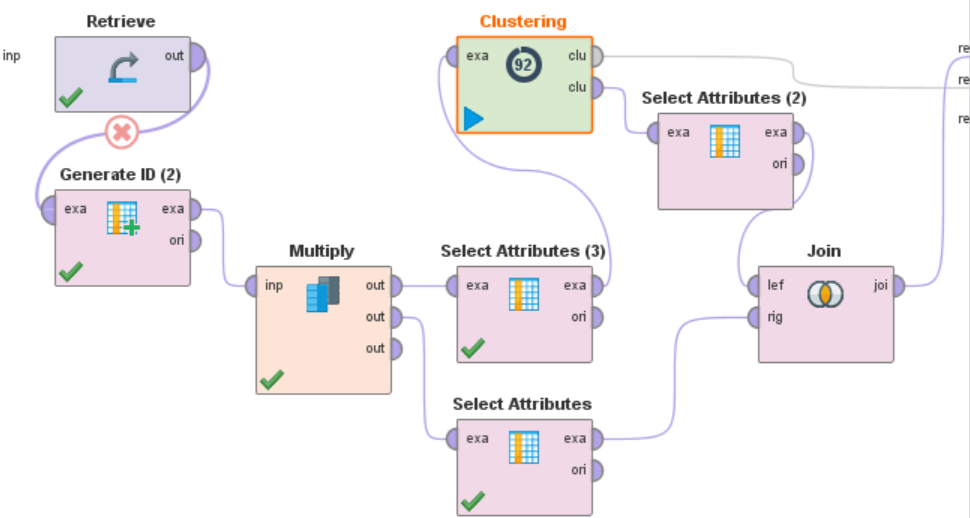
\includegraphics[width=0.9\textwidth]{ClusteringRapid.PNG}
		\caption{Process of k-means clustering}
		\label{fig: kclust}
		\vspace*{-2em}
	\end{figure}

	The Process, \Cref{fig: kclust}, contains the following steps:\\
	\begin{tabular}{r c l}
		\textbf{Retrieve} & : &  gives the data into the process \\
		\textbf{Generate ID} & : & creates an ID such that we can make the comparison\\
		 & & step at the end through joining the sets\\
		\textbf{Multiply} & : & creates two identical data sets\\
		\textbf{Select Attributes} & : &  troughs away the strata before the clustering step,\\
		& & everything except cluster and id after the clustering \\
		& & and just keeps id and strata for the join step\\
		\textbf{Clustering} & : &  runs the k-means clustering algorithm. The number of \\
		& & Clusters has to be fixed \\
		\textbf{Join} & : & For comparing the clustering result and the strata we \\
		& & join the two filtered data sets by the id \\
	\end{tabular}
	
	In the clustering block, we can choose between different distance measures and maximal step numbers. We keep the default configuration and choose the mixed euclidean distance measure.
%	We decide to concentrate on almost everywhere basic configurations and chose the squared euclidean distance in the mixed version.
\vspace*{-1em}
	\subsubsection{Gower Distance}\label{gower}, in contrast to the popular distance measures, can also handle the mixed data within the given dataset. The Gower distance measure distinguishes between three types of variables: binary, categorical and numerical.
%	When clustering data with algorithms such as \textit{k-means}, the distance between data points is usually calculated by measures such as the Euclidean or Manhattan norm.
%	These distance measures come with constraints though, since they are only defined for numerical variables. 
	%In the scope of this work, we are facing data points with mixed variable types.
	%, therefore we investigated the \textbf{Gower distance measure} as an appropriate measure to calculate an overall \textit{similarity} between mixed data points. 
%	\\ \textbf{Binary} variables, where two variables of value 0 are \textit{not} considered as match \cite{gower1971general}. In the scope of this work, the only considerable candidate for a binary variable would have been \textit{gender}. Though, during our research process, we concluded that the similarity measure for binary variables was not a suitable choice, as the distance does not match 0 values. Hence, we consider all variables, that are not explicitly numerical, as categorical variables.\\
%	\textbf{Categorical} variables form a set of unordered values and are comparable to ENUMs in programming languages.\\	
%	\textbf{Numerical} variables hold ordered numerical values that support arithmetic operations.
%	\subsubsection{Calculating the distances}
	The distance can be calculated as follows:
	
	Given two data points $x$ and $y$, each form a tuple of $v$ variables of arbitrary type, the similarity coefficient is given by
	\begin{equation}\label{eq1}
	S_{xy} = \sum_{k=1}^{v} s_{xy,k} / \sum_{k=1}^{v} \delta_{xy,k} 
	\end{equation} 
	where $s_{xy,k}$ denotes a \textit{score for the similarity} of the two variables at the $k$-th entry in the data points $x$ and $y$. Note, that the definition of the score depends on the
	%Timo nervt
	type of the variable, as defined below. In the divisor, $\delta_{xy,k}$ basically represents the possibility of comparing the two variables at index $k$, such that it evaluates to 1, if the two variables are comparable and to 0 if not. %PASS AUF
	For example, variables are not comparable, if values are undefined in the data points or the variable types do not match. Within this work, the dataset is complete, therefore, $\sum_{k=1}^{v} \delta_{xy,k}=v$. Thus, the similarity coefficient in \hyperref[eq1]{(2)} can be interpreted as the average value of all similarity scores. 
	With respect to the variable type, the similarity score $s_{xy,k}$ is defined as follows:\\
	\\ \textbf{Binary:} The score for binary variables is basically the result of an logical AND operation. As pointed above, 0 values are not considered as a match and even further, not considered to be comparable. Hence, the values result as in the table
		\begin{center}
			\begin{tabular}{l | c c c r}
				i & 1 & 1 & 0 & 0 \\
				j & 1 & 0 & 1 & 0 \\
				\hline
				$s_{xy,k}$ & 1 & 0 & 0 & 0 \\
				$\delta_{xy,k}$ & 1 & 1 & 1 & 0
			\end{tabular}
		\end{center}	
	\textbf{Categorical:} The similarity score of categorical variables is 1, if the variables are completely identical in $x$ and $y$, and 0, if they differ.
	
	\textbf{Numerical:} For numerical variables, the similarity score is calculated by
		\begin{equation*}
		s_{xy,k} = 1 - \frac{\vert x_k - y_k \vert}{range(k)}
		\end{equation*}
		where $range(k)$ is the total range of values, that the numerical variable at index $k$ can accept. This can be a global maximum of acceptable values for variable $k$, or chosen on the basis of the dataset.
		
		
	\subsection{Supervised learning}
	
	\subsubsection{Decision Trees} are a good manner to figure out, which parts of the data set have the most influence on the decision. Therefore labelled data is needed and we have given the strata. We used again RapidMiner for building trees based on different data sets. 
	
	\begin{figure}[!htbp]
		\centering
		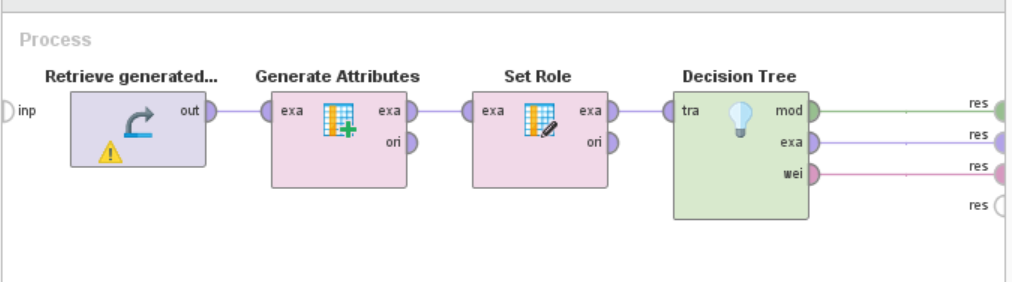
\includegraphics[width = 0.9\textwidth]{DecisionTreeRapidModel.PNG}
		\caption{Process for decision trees in RapidMiner}
		\label{fig: RapDec}
	\end{figure}
	
	RapidMiner does the following steps, illustrated in \Cref{fig: RapDec}:
	
	\begin{tabular}{r c l}
		\textbf{Retrieve} & : & includes the dataset\\
		\textbf{Select Attributes} & : & makes it possible to or have a look at grouped\\
		&& strata or normal strata\\
		\textbf{Set Role} & : & gives strata the label role, so that the decision tree\\
		&& has those as leafs\\
		\textbf{Multiply} & : & clones the data set \\
		\textbf{Decision Tree} &: & creates the decision tree\\
		\textbf{Apply Model} & : & creates the labelled data set for the \textbf{Performance} step\\
		\textbf{Performance} & : & gives the performance result of the created model\\
	\end{tabular}
	
	Furthermore we choose information gain as splitting criterion (minimal gain 0.1) and a confidence of 0.25. Other configurations do not show different results.
	
	\subsubsection{Neural Net}
	% TODO
	% like k-means
	are based on biology. In detail based on the neurons and synapses within the human brain. There a neuron fires to any further connected neurons, if a weighted sum minus a bias value is above a certain threshold.
%	The individual weights and biases are learned by the net.
	Through iteration-wise computing the result and comparing it to the expected outcome, called label and the use of various machine learning techniques the net is able to adjust the weights and biases \cite{neuralNet}.
	
	\begin{figure}[H]
		\centering
		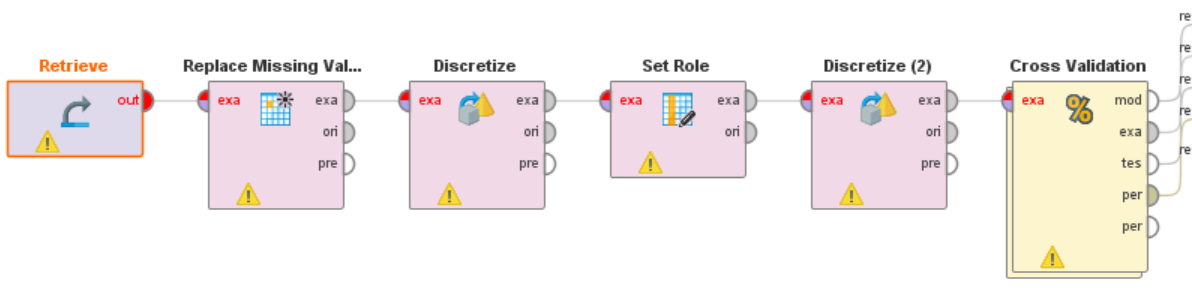
\includegraphics[width = 0.9\textwidth]{RapidNN.PNG}
	\end{figure}
		\begin{tabular}{r c l}
		\textbf{Retrieve} & : & includes the dataset\\
		\textbf{Replace Missing Values} & : & ensure applicable data\\
		\textbf{Discretize} & : & translates numerical to nominal data \\
		\textbf{Set Role} & : & gives strata the label role, so that the decision tree\\
		&& has those as leafs\\		
		\textbf{Cross Validation} & : & models the neural network \\
	\end{tabular}
	

%	\subsection{Preprocessing}\label{sec: proprocessing}
	In order to classify the given data into smaller test sets or mask different aspects, we have to perform some analysis.\\
	We observe that even though we have 124979 individual lines defining a movement, there is one line defining a \texttt{NotANumber}-exception and therefore gets neglected for further usage.	\\
	We provide the \texttt{testDataGenerator} python script. Through flags and input arguments, the script is able to create all test sets used by our clustering and neural net approaches.\\
	We observe the following distribution over the whole dataset:\\
	
	\vspace*{-3em}
	\begin{figure}[H]
		\centering		
		\setlength\tabcolsep{.2cm}
		\begin{tabular}{c|ccccccc}
			strata &  1   &   2   &   3   &  4   &  5   &  6   & $\Sigma$ \\ \hline
			abs   & 6963 & 52265 & 49404 & 8772 & 5536 & 2038 &  124978  \\
			\%   & 5.57 & 41.82 & 39.53 & 7.02 & 4.43 & 1.63 &   100
		\end{tabular}
		\vspace*{-2.5em}
		\label{table: distribution normal}
	\end{figure}
	There is an upper bound on equal distribution through strata 6. It has at most 2038 individual elements.
	Furthermore we have to make sure that two different data points, which belong to the very same person, are assigned to the same cluster. To do so, we compute the value \texttt{ID}, which identifies each person and can be used to combine movements that are considered to be from the same person. I.e. two movements correspond with the very same person, if and only if they are consecutive in the original dataset and have the same strata, age and gender. This approach is taken since the surveys are concatenated sequentially and it is unlikely, that multiple consecutive movements with same strata, age, gender belong to two different persons.\\
	
	\vspace*{-3em}
	\begin{figure}[H]
		\centering
		\setlength\tabcolsep{.2cm}
		\begin{tabular}{c|ccccccc}
			strata &  1   &   2   &   3   &  4   &  5   &  6  & $\Sigma$ \\ \hline
			abs   & 3153 & 23367 & 21418 & 3497 & 2083 & 595 &  54113   \\
			\%   & 5.83 & 43.18 & 39.58 & 6.46 & 3.85 & 1.1 &   100
		\end{tabular}
		\vspace*{-2.5em}
	\end{figure}
	Following, we introduce vectors representing single persons. Since strata 6 is the smallest strata with 595 persons, it limits the size of an equally distributed dataset where each data point coincides with one person.\\
	
	\textbf{Stratified Person Data}\label{subsubsec: person vector data}\\
	As stated before, instead of simple IDs for every person we expand the parsing by using a data encapsulating in a class called \texttt{Person}. This class stores the ID, the parameters defining a person (c.f. \Cref{sec: proprocessing}), and all movements from that person.\\
	Then we are able to compute the following vector, with 850 entries, for further usage, that combines all movements of the person:
	\begin{align*}
	\underbrace{\#o_1, \dots, \#o_{413}, \#d_1, \dots, \#d_{413}}_{2\cdot 413} ,
	\underbrace{\mathit{AM}, \mathit{MD}, \mathit{PM}, \mathit{MN}}_{4}, 
	\underbrace{\#r_1, \dots, \#r_7}_{7}, \\
	\underbrace{\#\mathit{MoT}_1, \dots, \#\mathit{MoT}_7}_{7}, \underbrace{\mathit{S_{Dest}}, \mathit{S_{Dist}}, \mathit{G}, \mathit{A} ,\mathit{strata}, \mathit{strataGrouped}}_{6}
	\end{align*}
	with the following abbreviations ($1 \le i \le 413$, $1 \le j \le 7$):
	\begin{figure}[H]
		\centering
		\hspace*{-.3cm}
		\begin{subfigure}{0.50\textwidth}
		\begin{itemize}
			\setlength{\itemindent}{.4cm}
			\item[$o_i$:]  the $i$-th origin data point
			\item[$d_i$:]  the $i$-th destination data point
			\item[$\mathit{AM}$:] movements at time stamp AM
			\item[$\mathit{MD}$:] movements at time stamp MD
			\item[$\mathit{PM}$:] movements at time stamp PM
			\item[$\mathit{MN}$:] movements at time stamp MN
			\item[$r_j$:] the $j$-th reason
		\end{itemize}
	\end{subfigure}\hspace*{1cm}
	\begin{subfigure}{0.48\textwidth}
	\begin{itemize}
			\item[$\mathit{MoT}_j$:] the $j$-th mean of transportation
			\item[$\mathit{S_{Dest}}$:] sum of all durations
			\item[$\mathit{S_{Dist}}$:] sum of all distances
			\item[$\mathit{G}$:] the gender
			\item[$\mathit{A}$:] the age
			\item[$strata$:] the strata (used for comparison)
			\item[$strataGrouped$:] the aggregated stratas
		\end{itemize}
	\end{subfigure}
	\end{figure}


	
	\section{Results}
		
	\subsection{Natural Clusters} \label{subsec: classification}
	
	%Miriam Clustering
\setlength{\parindent}{0em}
The first question was: is it possible without knowing the social classes to reproduce them based on the movement data. Therefore we wanted to look for clusters and compare those with the strata. Also we had a look if the possibly found clusters have special properties.

\subsubsection{Clustering with RapidMiner}

RapidMiner has different Modules for Clustering already implemented. We decided to concentrate on the k-means clustering algorithm.
\begin{figure}[!htbp]
\centering
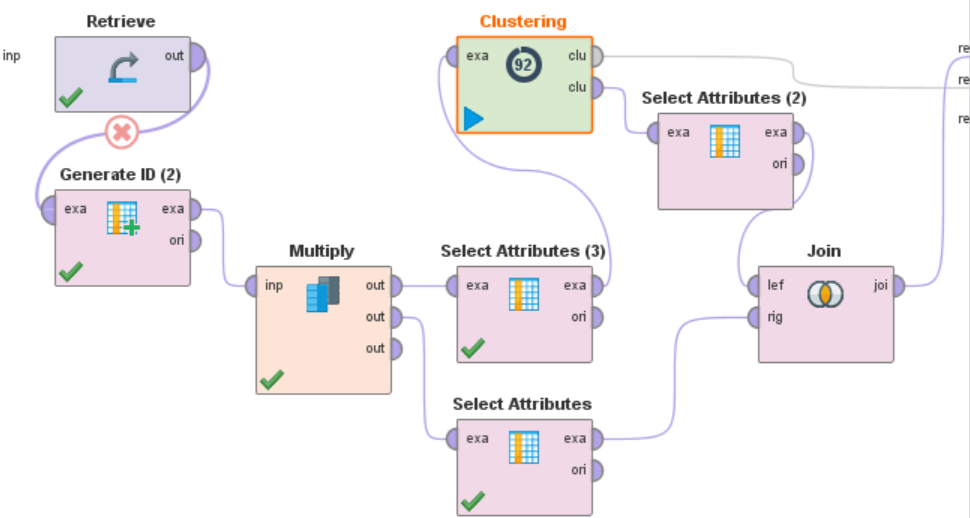
\includegraphics[width=0.9\textwidth]{ClusteringRapid.PNG}
\caption{Process of k-means clustering}
\label{fig: kclust}
\end{figure}


The Process, figure \ref{fig: kclust}, contains the following steps:
\begin{description}
	\item[Retrieve] gives the data into the process. 
  \item[Generate ID] creates an ID such that we can make the comparsion step at the end through joining the sets
  \item[Multiply] creates two identical data sets
  \item[Select Attrbiutes] thoughs away the strata before the clustering step, everything behalve cluster and id after the clustering and just keeps id and strata for the join step
	\item[Clustering] runs the k-means clustering algorithm. The number of Clusters has to be fixed.
	\item[Join] For comparing the clustering result and the strata we join the two filtered data sets by the id
\end{description}

In the clustering block we can chose between different distance measures and maximal step numbers. We decided to concentrate on almost everywhere basic configurations and chose the squared euclidean distance in the mixed version.

In the first step we tried to cluster the \textbf{Original Data} in \textbf{6 Cluster}. Therefore we retrieved the original data set in RapidMiner and chose k as 6.

\ref{fig:OrgDist}. 
\begin{figure}[!htbp]
\centering
\begin{subfigure}{.5\textwidth}
  \centering
  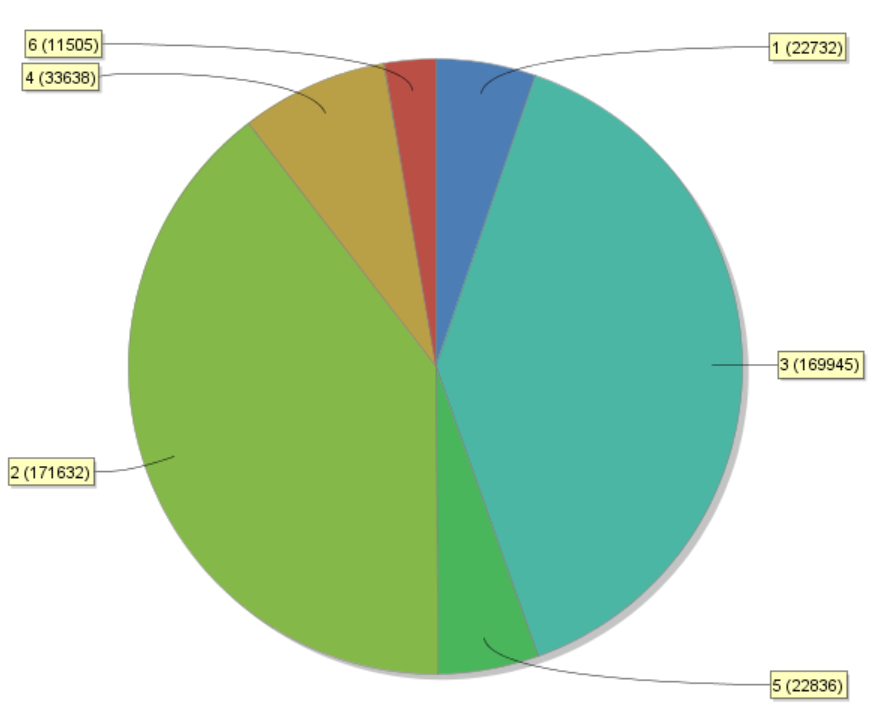
\includegraphics[width=.8\linewidth]{ClusterOrigRapidStrata.PNG}
  \caption{Strata}
  \label{fig:OrgSt}
\end{subfigure}%
\begin{subfigure}{.5\textwidth}
  \centering
  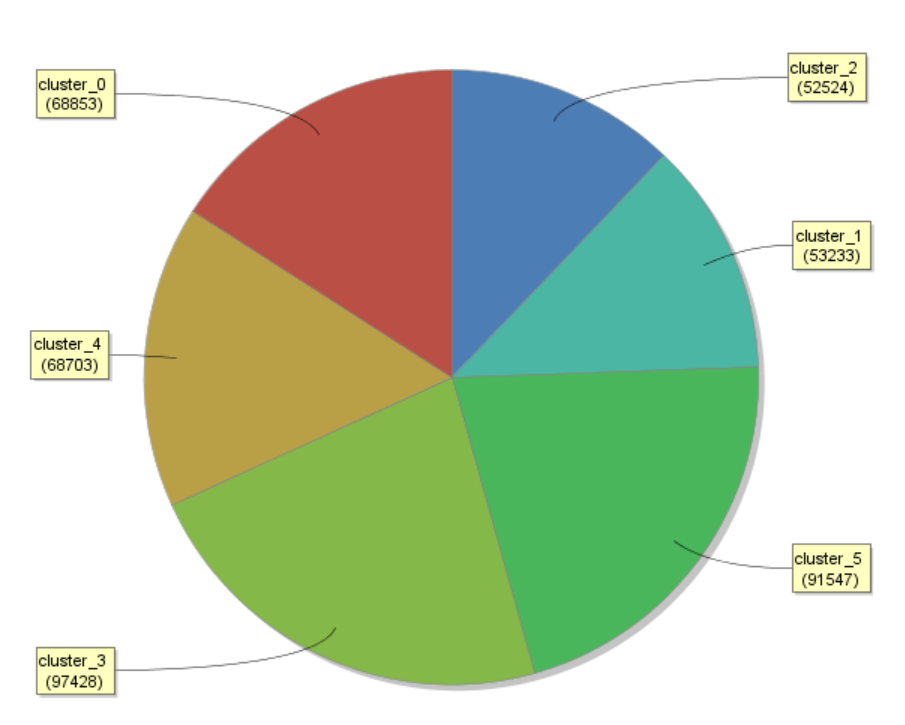
\includegraphics[width=.8\linewidth]{ClusterOrigRapidCluster.PNG}
  \caption{Cluster}
  \label{fig:OrgCl}
\end{subfigure}
\caption{Distribution of original data}
\label{fig:OrgDist}
\end{figure}

In figure \ref{fig:OrgDist} is the result to see of the first try. Figure \ref{fig:OrgSt} shows the strata distribution as pie chart and \ref{fig:OrgCl} the resulted cluster distribution. It can already been seen, that the distributions are not similar. In the next step we tried it with more steps, but the result was not looking better.

We asked ourselfs, if 6 cluster is not too fine, so we searched for \textbf{3 clusters} in the next step. The idea is to combine two stratas in 1, such that we just have 3 stratas left.
\begin{figure}[!htbp]
\centering
\begin{subfigure}{.5\textwidth}
  \centering
  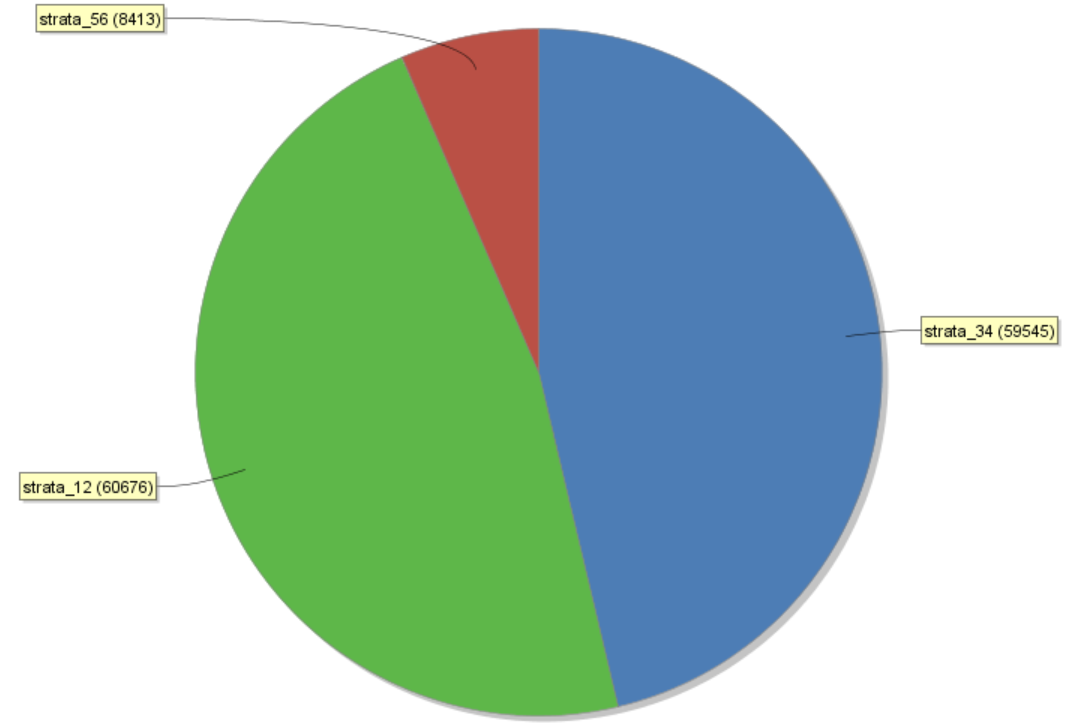
\includegraphics[width=.8\linewidth]{ClusterOrigRapidStrata2Cluster.PNG}
  \caption{Strata}
  \label{fig:OrgSt}
\end{subfigure}%
\begin{subfigure}{.5\textwidth}
  \centering
  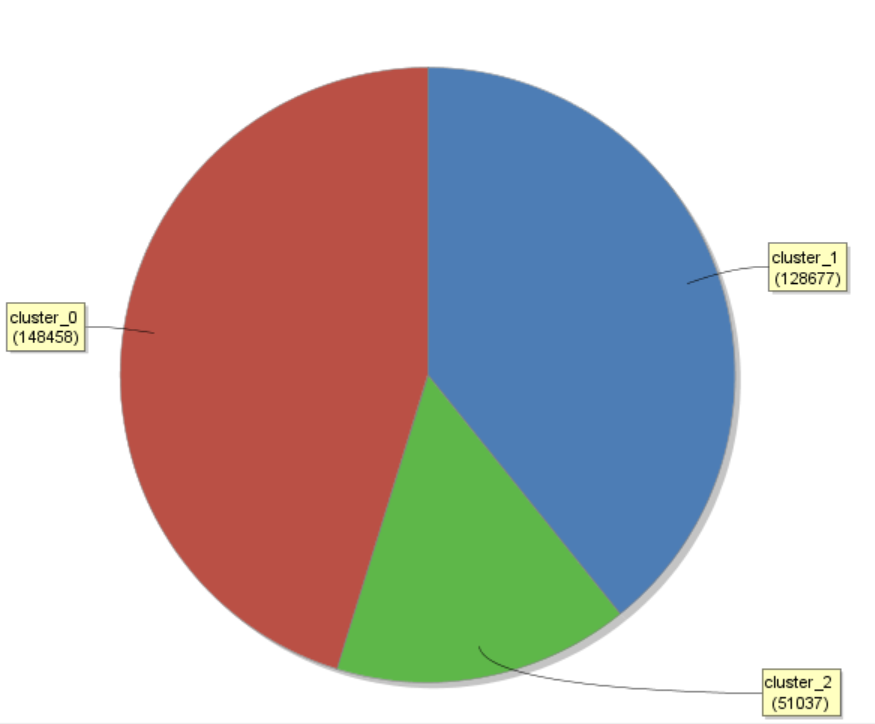
\includegraphics[width=.8\linewidth]{ClusterOrigRapidCluster2Cluster.PNG}
  \caption{Cluster}
  \label{fig:OrgCl}
\end{subfigure}
\caption{Distribution of original data for just 3 clusters}
\label{fig:OrgDist3Cl}
\end{figure}

\begin{figure}[!htbp]
\centering
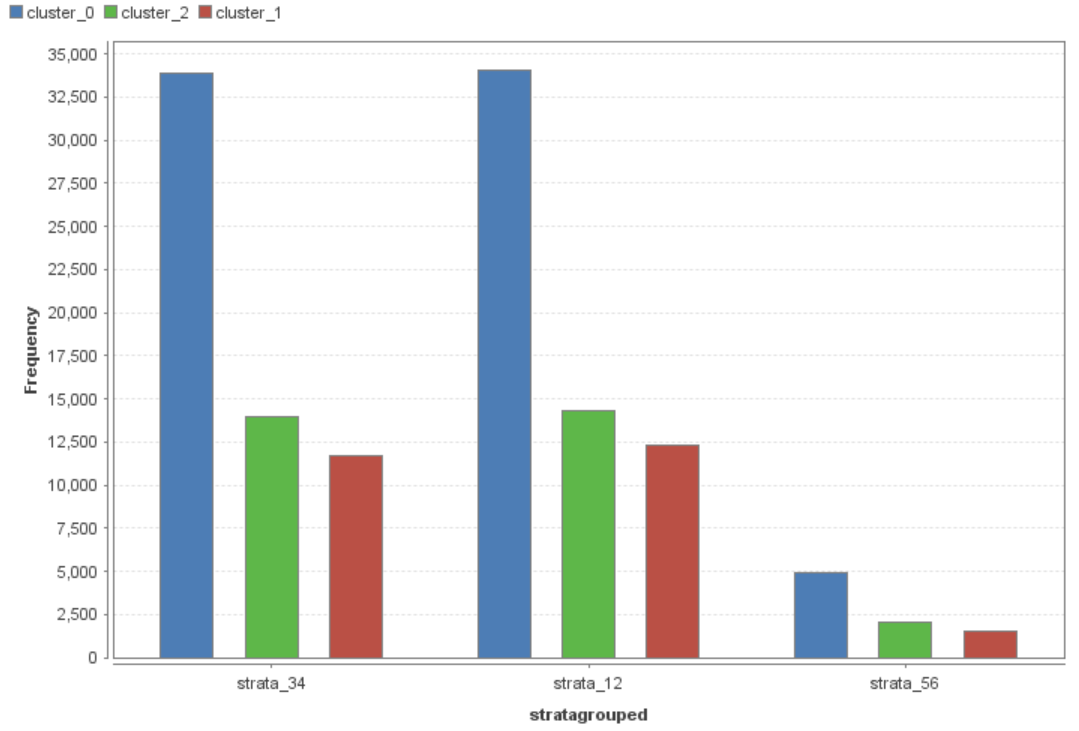
\includegraphics[width=0.9\textwidth]{ClusterOrigRapidDistribution2Cluster.PNG}
\caption{Distribution of the clusters in between the grouped strata}
\label{fig:Groupdist}
\end{figure}

After having a look at the pie charts, \ref{fig:OrgDist3Cl} and so the distribution in between the variable it seems to be a better result, so we had a look at the cluster distribution in the 3 grouped stratas, \ref{fig:Groupdist}. This figure shows clearly, that there is no real correlation between strata 

\begin{figure}[!htbp]
\centering
\begin{subfigure}{0.9\textwidth}
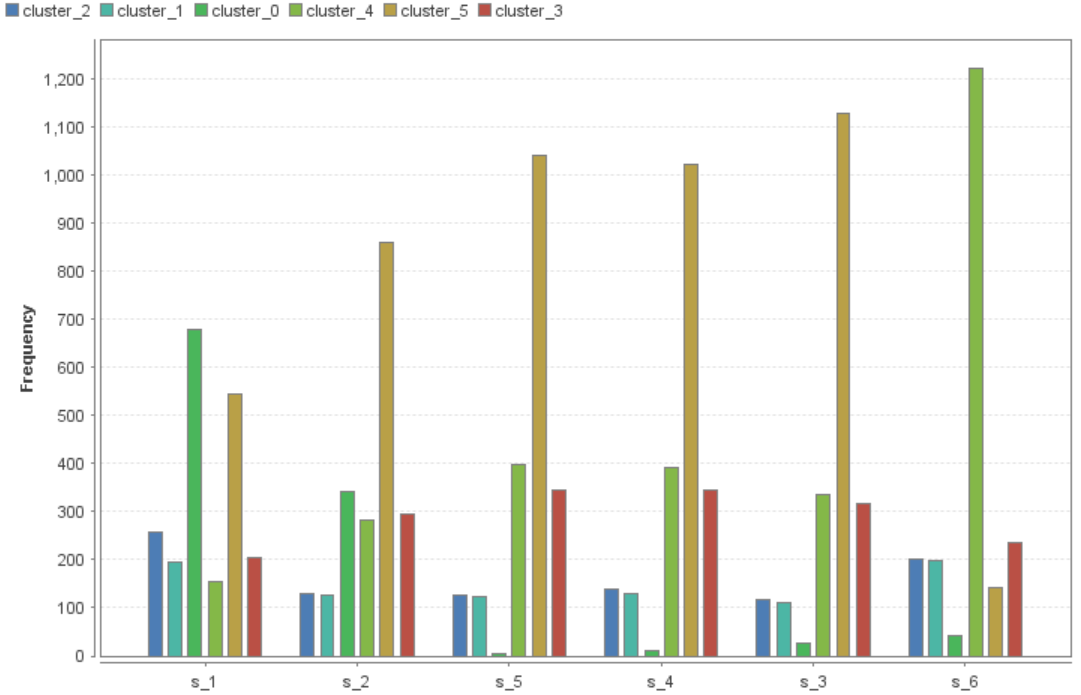
\includegraphics[width=\linewidth]{ClusterOrigRapidDistribution2038eq.PNG}
\caption{For 6 clusters}
\label{fig:2038_6}
\end{subfigure}
\begin{subfigure}{0.9\textwidth}
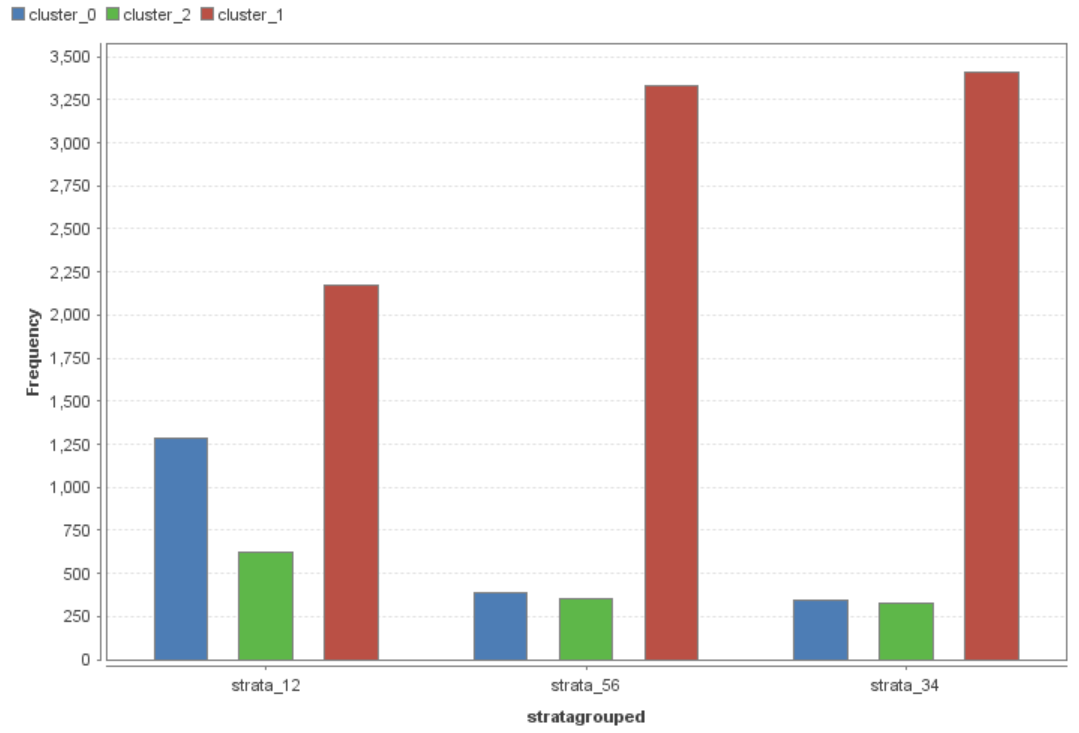
\includegraphics[width=\linewidth]{ClusterOrigRapidDistribution2038eq2.PNG}
\caption{For 3 clusters}
\label{fig:2038_3}
\end{subfigure}
\caption{Distribution of the clusters in between the strata}
\label{fig:2038_Clust}
\end{figure}

The result for different datasizes and equal distribution of the stratas does not change the result. The biggest equal distributed dataset has 2038 data rows for every strata and 4076 in between the grouped strata. In figure \ref{fig:2038_Clust} the two clustering results can be seen. Again we could not really see a significant correlation.

\textbf{Stratified Person Data}

After those not really convincing results we applied the process on the stratified person data, because those represented the movement of one person.

\begin{figure}[h]
\centering
\begin{subfigure}{.5\textwidth}
  \centering
  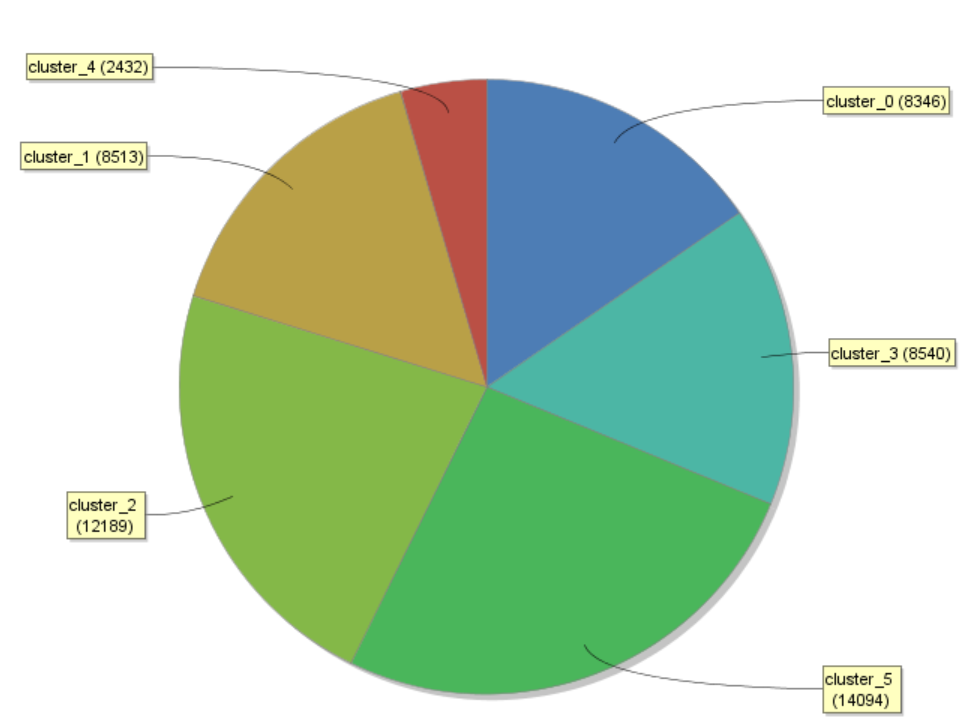
\includegraphics[width=.9\linewidth]{vectorclusteringcluster.PNG}
  \caption{Strata}
  \label{fig:VecSt}
\end{subfigure}%
\begin{subfigure}{.5\textwidth}
  \centering
  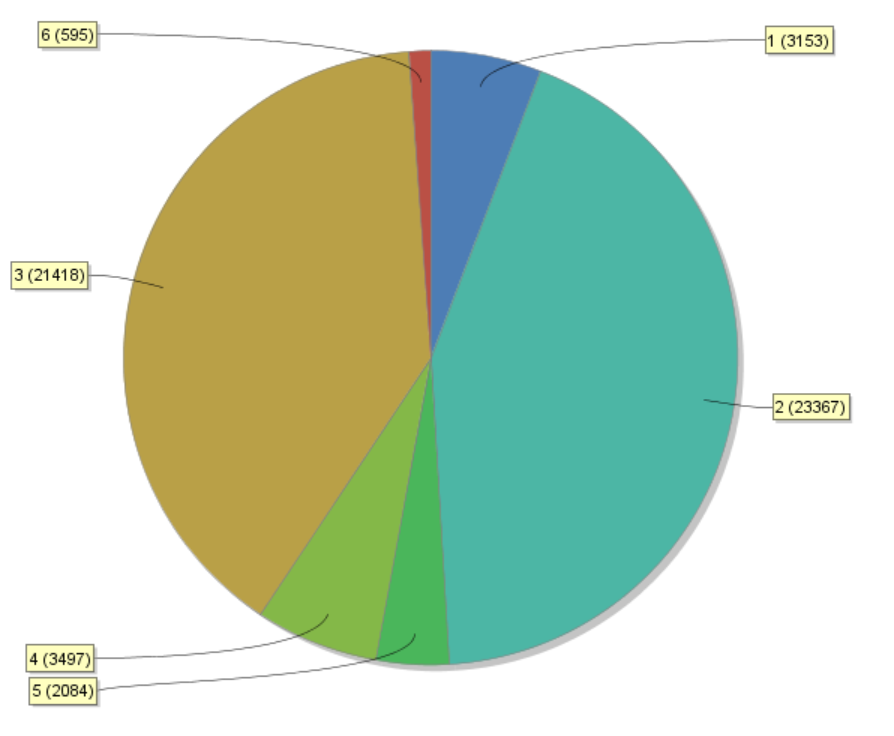
\includegraphics[width=.9\linewidth]{vectorclusteringstrata.PNG}
  \caption{Cluster}
  \label{fig:VecCl}
\end{subfigure}
\caption{Distribution of stratified person data}
\label{fig:VecDist}
\end{figure}

\begin{figure}[!htbp]
\centering
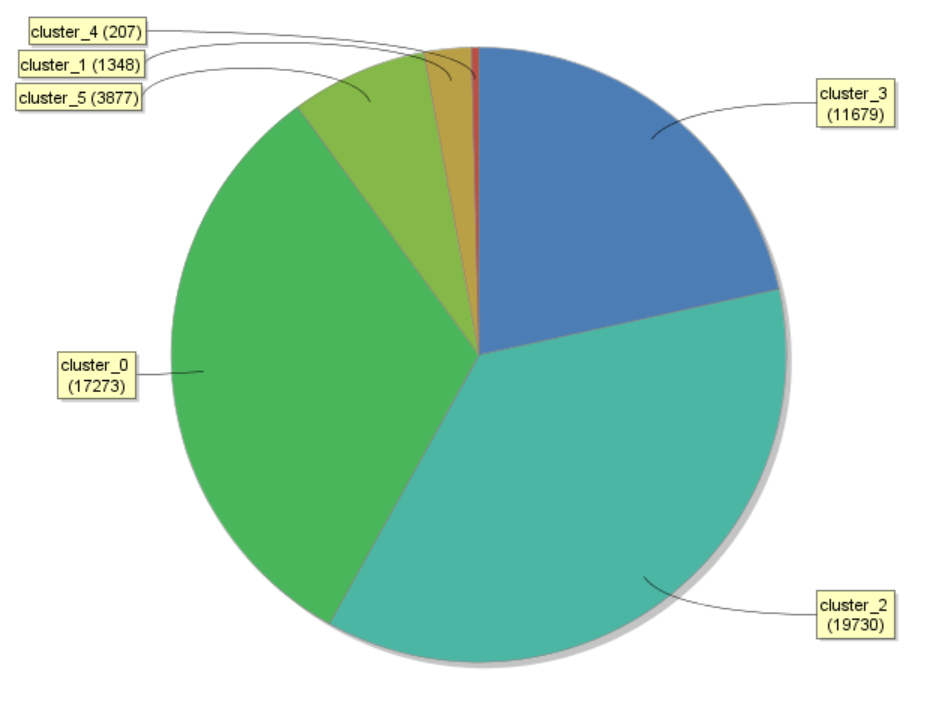
\includegraphics[width=0.3\textwidth]{vectorclusteringcluster1000.PNG}
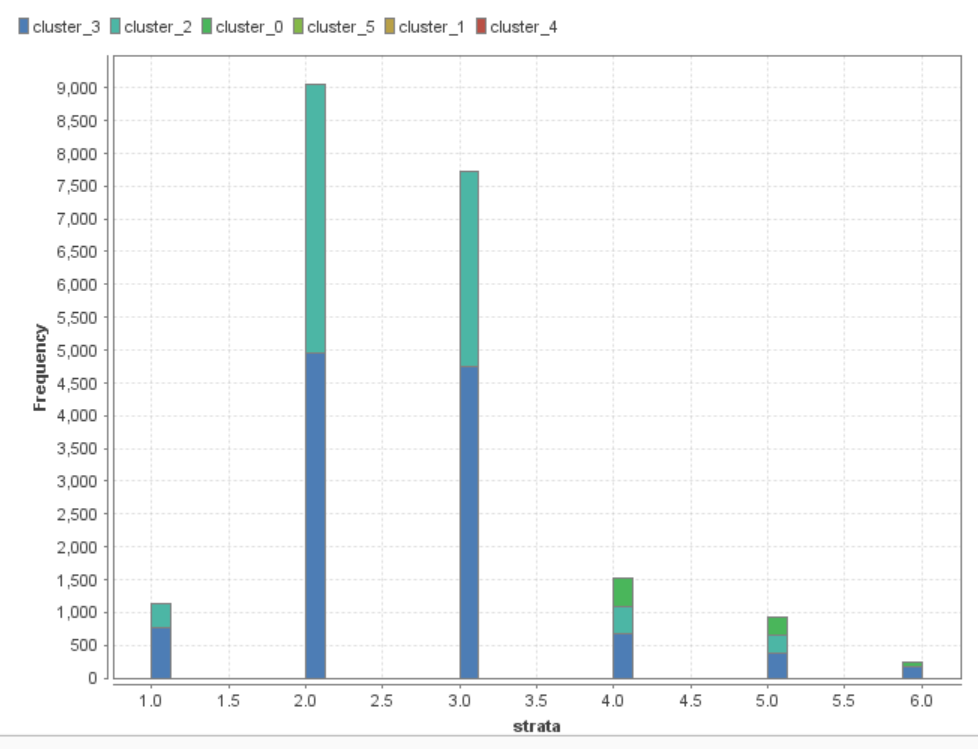
\includegraphics[width=0.69\textwidth]{vectorClustering1000.PNG}
\caption{1000 steps clustering in 6 clusters}
\label{fig:1000vect}
\end{figure}

The results for the whole data set without equalization are shown in figure \ref{fig:2038_Clust}. We changed the number of steps to 1000 for comparsion and the result, \ref{fig:1000vect}, let us assume, that 3 clusters better would fit. 


So we applied the process on the \textbf{stratified person data} and searched for \textbf{3 clusters}. We directly run the algorithm 1000 steps.

\begin{figure}[!htbp]
\centering
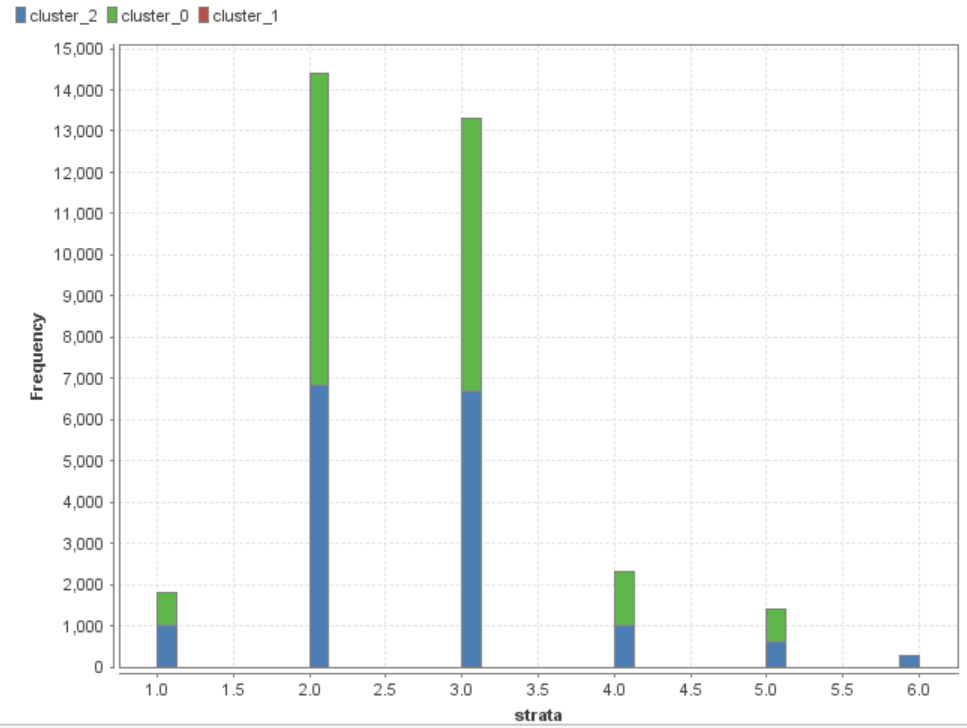
\includegraphics[width=0.69\textwidth]{vectorClustering31000.PNG}
\caption{1000 steps clustering in 3 clusters}
\label{fig:1000vect3}
\end{figure}

Figure \ref{fig:1000vect3} shows clearly, that again no correlation can be found. Furthermore we applied this for the different datasets we generated, but the result was always similar.


%PCA??

	\setlength{\parindent}{0em}
\subsection{Decision Tree} \label{subsec: decisiontree}
Decision trees are a good manner to figure out, which parts of the data set have the most influence on the decision. Therefore labeled data is needed and we have given the strata. We used again \textbf{RapidMiner} for building trees based on different data sets. 

\begin{figure}[!htbp]
\centering
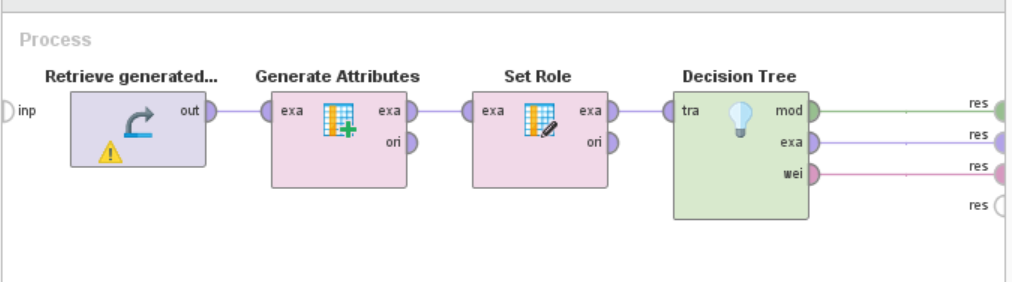
\includegraphics[width = 0.9\textwidth]{DecisionTreeRapidModel.PNG}
\caption{Process for decision trees in RapidMiner}
\label{fig: RapDec}
\end{figure}

RapidMiner does the following steps, to see in figure \ref{fig: RapDec}:
\begin{description}
	\item[Retrieve] includes the dataset
	\item[Select Attributes] makes it possible to or have a look at grouped strata or normal strata
	\item[Set Role] gives strata the label role, so that the decision tree has those as leafs
	\item[Multiply] clones the data set 
	\item[Decision Tree] creates the decision tree
	\item[Apply Model] is used creates the labeled data set for the \textbf{Performance} step
	\item[Performance] gives the performance result of the created model
\end{description}

Furthermore we choose information gain as splitting criterium (minimal gain 0.1) and a confidence of 0.25. Other configuration does not show different results.

In the first step we applied the process on the whole data set and the resulting tree was just the leaf "strata 2". So we tried it with different other data sets and the best result we got was for \textbf{stratified person data} equally distribute and just 200 in every strata group.

\begin{figure}[!htbp]
\centering
\begin{subfigure}{0.9\textwidth}
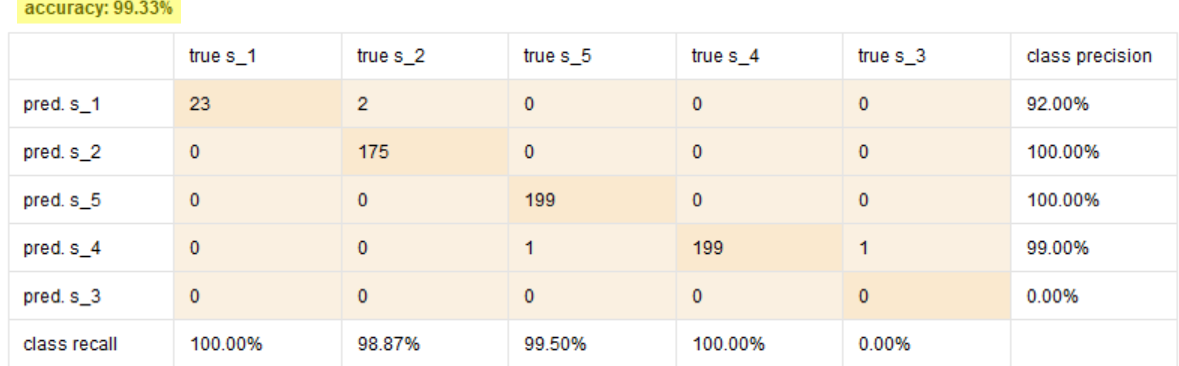
\includegraphics[width = \linewidth]{Dec200eqPrec.PNG}
\caption{200 in every strata}
\label{fig:decvec200}
\end{subfigure}
\begin{subfigure}{0.9\textwidth}
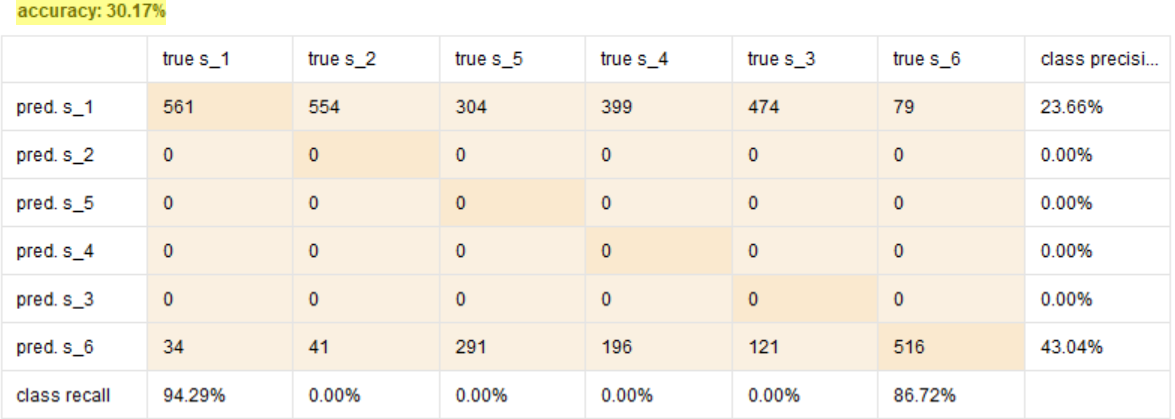
\includegraphics[width= \linewidth]{decvec585pre.PNG}
\caption{585 in every strata}
\label{fig:DecVec585}
\end{subfigure}
\caption{Performance for stratified person data}
\label{fig:DecVec}
\end{figure}

In figure \ref{fig:DecVec} the best and worst outcome can be seen for 6 clusters. For all othe configurations the outcome was similar, so just small data sets had a good result and big data sets had no really good result for our question, such that we still had no explicit result with which we could work.
	
	

\textbf{Neural Net} \label{subsec: neural net}\\
	In this section we want to further improve the accuracy of predicting the strata of one person by using neural networks. Like in the previous section, where we used decision trees, we need ground truth to be able to train the neural networks. For all the neural net computations we consider person vector data sets of different sizes (c.f. \Cref{sec: proprocessing}).\\	
	We do this, because results on the normal datasets had an unacceptable performance, since only single movements and not complete paths of individuals are considered. An example training and performance measure is given in \Cref{fig: NN without vector}, where unprocessed data is used. The performance is measured using 10-fold cross validation, i.e. the data is split into 10 subsets, where in each iteration exactly one data set is used as test set and the other 9 as training set. The average value of those accuracy values leads to the total accuracy of the neural net.

	
	In the following we consider 3 neural nets $\mathcal{N}_1,\mathcal{N}_2$ and $\mathcal{N}_3$, all having 4 hidden layers, 50 epochs and 10 iterations.	
	We call the aggregated strata sets $\mathcal{N}_i^\star$, for $i \in \{5,10,20\}$ denoting the number of neurons. This builds a superset of the original stratas and since the stratas themselves are logically connected, this task should be easier to fulfill.\\
		\begin{figure}[H]
		\vspace*{-1em}
		\centering
		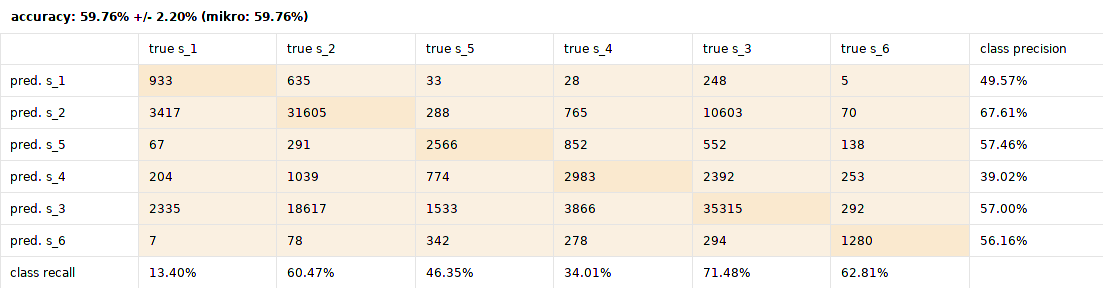
\includegraphics[scale = 0.4]{src/pic/NN_without_vector.png}
		\caption{An example of a neural net trained without person vector data.}
		\label{fig: NN without vector}
	\end{figure}
	\vspace*{-1.5em}
	
	For each neural net we are using equally distributed data sets with 100, 200 and the maximal amount of 595 individuals per strata. For every neural net and every set size, we perform 5 independent runs and calculate the average over those accuracy values in order to have a sophisticated, comparable statement. 
	\setlength\tabcolsep{.2cm}
	\begin{figure}[H]
		\centering
		\begin{tabular}{|c|c|c|c|c|c|}
			\hline
			&   \#    &        & \multicolumn{3}{c|}{Set size} \\
			Name           & Neurons &   AG   &  100  &  200  &      595      \\ \hline
			$\mathcal{N}_5$      &    5    & \xmark & 60.03 & 59.92 &     60.18     \\
			$\mathcal{N}_5^\star$   &    5    & \cmark & 87.6  & 89.7  &     71.05     \\
			$\mathcal{N}_{10}$    &   10    & \xmark & 75.83 & 73.54 &     69.56     \\
			$\mathcal{N}_{10}^\star$ &   10    & \cmark & 92.93 & 93.48 &     74.58     \\		
			%		$\mathcal{N}_{10}^\star$ &   10    & \cmark & 88.33 {\small $\pm$7.49} & 90.67{\small $\pm$2.81} & 92.14 {\small $\pm$ 2.59} \\
			$\mathcal{N}_{20}$    &   20    & \xmark & 75.45 & 71.14 &     61.87     \\
			$\mathcal{N}_{20}^\star$ &   20    & \cmark & 92.87 & 94.4  &     78.32     \\ \hline
		\end{tabular}
		\caption{The accuracy values of the neural nets}
		\label{tab: nn-accuracy}
		% mittels deep-learning-vector-average
	\end{figure}
	
	%TODO: recompute
	The size of larger nets, in terms of neurons, is counter-productive, since, if we take 50 neurons per layer, we have $14 \cdot 50^4 \cdot 6 < 849 \cdot 50^4 \cdot 6 \approxeq 31.837.500.000$ synapses for which the input dataset would be too small to perform sufficient training.\\
	
	\section{Conclusion} \label{sec: observation}
	%	TODO (1 page)
	%	TODO: restructure. Have like 3 parts
	%	The greater the population, the more the borders between the stratas blur. 
	As an overall result we observe, that we can not determine the strata based on the information we have.
	Using various datasets, we witness, that having equally distributed datasets leads to an overall higher accuracy. This rules out the bias observed in the original data, where strata 2 and 3 are very dominant (c.f. \Cref{table: distribution normal}), but also reduces the set size from originally 124978 to $6*2038=12228$ entries equally distributed over all stratas.\\
	During clustering we observe, that using a different distance measure formula would not lead to a huge difference. Also, we detect that reducing the number of clusters leads to better results, but decreases the significance of the statement, that could be made.\\
	Using a different neural net architecture will most likely not chance the accuracy value drastically. As stated, more complex nets need more training data, which is restricted for the reasons mentioned above.\\
	What we can observe is, that using the stratified vectors, we are able to increase the performance and accuracy, but still have no sufficient predictions. Therefore we see: the more data we have, the higher the variance within the stratas is. We cannot draw lines to distinguish between different stratas. Data points, which were outliers in the smaller sets, are now not considered to be outliers, because many others have the same characteristics. So the lines, we were able to draw for smaller datasets, are blurring.\\ %TODO: letzter satz doof	-> hihi	
	
	
		\section{Discussion} \label{sec: discussion}
%	\begin{itemize}
%		\item repr. working day
%		\item over/under std's
%		\item indiv. of lifestyle
%		\item inv. behaviour in same strata
%	\end{itemize}
	Regarding the results, of not predicting the strata and also not observing any meaningful clusters throughout the data in given and stratified form, we though about various aspects having an impact on the movement. We state 4 main influencing aspects, explaining the variance throughout the data.
	
	\subsection{Representativity of the day}
	The day the data was collected on (c.f. \Cref{sec: introduction}) is not mentioned. Therefore we cannot infer, that it is representative. The people, asked to enter their movement, could have a exceptional day, like a vacation day, a doctors appointment or a broken car and therefore behave different from a usual day. \\
	Also the day itself is not mentioned, so we do not have information, if it was even a working day or a weekend. This influences the behavior drastically.
	
	\subsection{People living over/under standards}
	There are a lot of people spending more or less money than they actually have. So for example there are people not earning a lot of money, but still having a car. Or people earning a lot, but spend it just on holidays or save it for bad times.
	
%	In Liebe
%	deine Miriam

	\subsection{Individuality of lifestyle}
	Obviously, people are individual in their way of life. So there are people, with enough money to buy for example a car, but refuse to in order to reduce CO$_2$ emission, or simply do not like driving. On the other end of the spectrum, some people, who have little money, still own and drive a car daily in order to go to work, since they cannot afford an other apartment.\\
	One can think of multitude scenarios of people behaving different caused by their individuality.
	
	\subsection{Inverse behavior in a strata}
	As an example, take a look at the strata 6, which denotes the richest people considered. Their we have inter alia two groups: 
	\begin{enumerate}
		\setlength{\itemindent}{1cm}
		\item[1. Group]
		Hard working people, laboring 60+ hours per weak to earn their money. One can imagine that they have to move quite a lot since they are always busy.
		\item[2. Group]
		People, who are rich just by birth, which do not have the necessity to work or move at all. They could possibly stay home and do not have to leave at all.
	\end{enumerate} 
	Those two groups are completely opposite, but still belong to the same strata. Now also considering strata one, we can find the exact same movement behavior in there as well. Within the poorest there are people that are wandering around the town via feet or bike, since they have no objective, like work. Also there are people, who do not move at all, because of the same reason.	
	
	So we can see that based on the information we have, it is very unlikely to have a clear correlation between the given data and the strata. However, given more information about the previously mentioned aspects and more entries in general, there could be some kind of correlation to be found.\\
	Future work could include a component analysis of the decision tree and neural network in order to ascertain the influencing parts and therefore improve the data gathering. Also one could use different network visualization tools in order to infer patterns. An example would be to take the origin (destination) sectors as nodes, an edge, if there is a movement between, directed or undirected, and a different thickness or color gradient, based on the number of this edge being taken.\\
	
	Overall we can conclude that with the data we got, we are not able to find a correlation.
	
	
	\begin{thebibliography}{8}
		\bibitem{rich_do_not_rise_early}
		Lotero, Laura, et al. "Rich do not rise early: spatio-temporal patterns in the mobility networks of different socio-economic classes." Royal Society open science 3.10 (2016): 150654.
		
		\bibitem{strata_def}
		Hudson, Rex A. Colombia: A country study. Government Printing Office, 2010.
		
		\bibitem{gower1971general}
		Gower, John C,
		\emph{A general coefficient of similarity and some of its properties},
		Biometrics, pp. 857-871,
		1971.
		
		\bibitem{data_mining}
		Han, Jiawei and Pei, Jian and Kamber, Micheline,
		\emph{Data mining: concepts and techniques},
		Elsevier, pp. 444-454,
		2011.
		
		\bibitem{population_number}
		Estimates and projections of the total national, departmental and municipal population by area 1985-2020 (XLS). NADS. Retrieved 1 September 2014.
		
		\bibitem{neuralNet}
		Nasrabadi, Nasser M. "Pattern recognition and machine learning." Journal of electronic imaging 16.4 (2007): 049901.
	\end{thebibliography}
\end{document}
